
\subsection{Background}
The first paradigm used to solve the VLSI optimization problem is Constraint Programming (CP),
developed using MiniZinc as modeling language.
Starting from a base model following the constraints discussed in Section \ref{sec:shared_constraints},
we added: rotation variables $r_i$, symmetry breaking constraints and search strategies. We have a model
for each combination of the previous elements.
To test different behaviour of solvers we chose to run each model on both Chuffed and Gecode solvers.
\colorbox{BurntOrange}{TODO: check last sentence}

% % % % % % % % % % % % % % % % % % % % % % % % % % % % % % % % % % % % % % % % % % % % % % % % % %

\subsection{Notation} \label{sec:CP_notation}
In CP we tried to break also the symmetries related to \textit{virtual} circuits, but we decided to
keep only the simplest ones for efficiency reasons, as anticipated in Section \ref{sec:symmetries}.

This section is mainly needed to introduce constants related to \textit{virtual} circuits:

\begin{align*}
  vc_{i,j} & \ =\ \text{\textit{virtual} circuit obtained from  } (i,j) \in CC      \\
  n\_vc\   & \ =\ \text{maximum number of \textit{virtual} circuits}                \\
           & \ =\ |CC| = \frac{nc!}{2! \cdot (nc - 2)!} = \frac{nc \cdot (nc-1)}{2} \\
  n\_rvc\  & \ =\ n\_vc + nc                                                        \\
  VC       & \ =\ \{ c_i\ |\ i \in [1,n\_vc] \}                                     \\
  VV       & \ =\ \{ (i,j)\ \in VC \times VC\ |\ i <j \}                            \\
  RVC      & \ =\ \{ c_i\ |\ i \in [1,n\_rvc] \}                                    \\
  % c_pairs &\ =\ [(i,j)\ |\ (i,j) \in CC]
\end{align*}

The first definition needs deeper explanation: a rectangle can be defined giving the position
of its bottom left and its top right corner. For a \textit{virtual} circuit the corners are the
bottom left corner of circuit $i$ and the top right corner of circuit $j$.
The maximum number of virtual circuits is then given by the number of possible combinations
(without repetition) of the circuit indexes grouped in pairs, which is also the cardinality of $CC$.



% % % % % % % % % % % % % % % % % % % % % % % % % % % % % % % % % % % % % % % % % % % % % % % % % %

\subsection{Functions \& Predicates} \label{sec:CP_functions_predicates}
The additional functions and predicates we define in this section will later be used in the models
that adopt symmetry breaking constraints or that allow the rotation of circuits. The other models
work with the constraints already defined in Section \ref{sec:shared_constraints}.

\paragraph{Functions}
\begin{align}
  vc\_x(vc_{i,j})\        =\  & min(x_i, x_j)                                                     \nonumber \\
  vc\_y(vc_{i,j})\        =\  & min(y_i, y_j)                                                     \nonumber \\
  vc\_width(vc_{i,j})\    =\  & max(x_i + w_i, x_j + w_j) - vc\_x(vc_{i,j})                       \nonumber \\
  vc\_height(vc_{i,j})\   =\  & max(y_i + h_i, y_j + h_j) - vc\_y(vc_{i,j})                       \nonumber \\
  r\_w(c) =\                  & bool2int(\neg\ is\_rotated_c) \cdot w_c + bool2int(is\_rotated_c) \cdot h_c
  \label{eq:CP_r_w}                                                                                         \\
  r\_h(c) =\                  & bool2int(\neg\ is\_rotated_c) \cdot h_c + bool2int(is\_rotated_c) \cdot w_c
  \label{eq:CP_r_h}
\end{align}

where $vc\_x(vc_{i,j})$, $vc\_y(vc_{i,j})$, $vc\_width(vc_{i,j})$ and $vc\_height(vc_{i,j})$
return respectively the $x_{vc_{i,j}}$, $y_{vc_{i,j}}$, $w_{vc_{i,j}}$ and $h_{vc_{i,j}}$ of
the \textit{virtual} circuit $vc_{i,j}$, while $r\_w(c)$ and $r\_h(c)$ check if circuit $c$
is rotated and update coherently $w_c$ and $h_c$.

\paragraph{Predicates}
% \begin{align*}
%     vc\_is\_valid(vc_{i,j})     &\leftarrow\    \bigwedge_{c \in C} &  (\neg(x_c < vc_x \land x_c + w_c > vc_x) \land
%                                                 \neg(x_c + w_c > vc_x + vc_w))                                  \\
%                                             &&  \lor                                             \\
%                                             &&  (\neg(y_c < vc_y \land y_c + h_c > vc_y) \land
%                                                 \neg(y_c + h_c > vc_y + vc_h))                                  \\
%     c\_equal\_dim\_symmetry &\leftarrow\        \bigwedge_{(c_1, c_2) \in CC} & (w_{c_1} == w_{c_2} \land h_{c_1} == h_{c_2})                   \\
%                                             &&  \rightarrow lex\_lesseq([x_{c_1}, y_{c_1}], [x_{c_2}, y_{c_2}]) \\ 
%     vc\_equal\_dim\_symmetry &\leftarrow\       \bigwedge_{(c, vc) \in C \times VC} & (vc\_is\_valid(vc) \land w_{c_1} == w_{c_2} \land h_{c_1} == h_{c_2})   \\
%                                             &&  \rightarrow lex\_lesseq([x_{c_1}, y_{c_1}], [x_{c_2}, y_{c_2}])     \\      
%     vv\_equal\_dim\_symmetry &\leftarrow\       \bigwedge_{(vc_1, vc_2) \in VV}
%                                             &   (vc\_is\_valid(vc_1) \land vc\_is\_valid(vc_2) \land                         \\
%                                             &&  \neg (vc_{1x} == vc_{2x}) \land \\
%                                             &&  vc_{1w} == vc_{2w} \land vc_{1h} == vc_{2h} \land \\
%                                             &&  (|vc_{1x} - vc_{2x}| \geq vc_{1w} \lor |vc_{1y} - vc_{2y}| \geq vc_{1h})) \\
%                                             &&  \rightarrow lex\_lesseq([vc_{1x}, vc_{1y}], [vc_{2x}, vc_{2y}]) \\
%     c\_consecutive\_on\_x(c_1, c_2) &\leftarrow  &   x_{c_1} + w_{c_1} == x_{c_2} \lor x_{c_2} + w_{c_2} == x_{c_1} \\
%     c\_consecutive\_on\_y(c_1, c_2) &\leftarrow  &   y_{c_1} + h_{c_1} == y_{c_2} \lor y_{c_2} + h_{c_2} == y_{c_1} \\
%     c\_can\_be\_swapped\_on\_x(c_1, c_2) &\leftarrow & c\_consecutive\_on\_x(c_1, c_2) \land y_{c_1} == y_{c_2} \land h_{c_1} == h_{c_2} \\
%     c\_can\_be\_swapped\_on\_y(c_1, c_2) &\leftarrow & c\_consecutive\_on\_y(c_1, c_2) \land x_{c_1} == x_{c_2} \land w_{c_1} == w_{c_2} \\ 
%     c\_consecutive\_symmetry &\leftarrow  \bigwedge_{(c_1, c_2) \in CC} & (c\_can\_be\_swapped\_on\_x(c_1, c_2) \rightarrow lex\_less([ x_{c_1} ], [ x_{c_2} ])) \land \\
%                                             &&  (c\_can\_be\_swapped\_on\_y(c_1, c_2) \rightarrow lex\_less([ y_{c_1} ], [ y_{c_2} ]))     
% \end{align*}
\begin{align}
  \text{vc\_valid}(vc_{i,j})      \leftarrow & \ \hspace{0.45cm} \bigwedge_{c \in C} \hspace{0.3cm} (\neg(x_c < vc_x \land x_c + w_c > vc_x) \land \neg(x_c + w_c > vc_x + vc_w))\ \lor      \nonumber           \\
                                             & \ \hspace{1.3cm} \lor (\neg(y_c < vc_y \land y_c + h_c > vc_y) \land \neg(y_c + h_c > vc_y + vc_h))                                                               \\
                                             & \nonumber                                                                                                                                                         \\
  \text{c\_eq\_dim\_sym}          \leftarrow & \ \bigwedge_{(c_1, c_2) \in CC} (w_{c_1} == w_{c_2} \land h_{c_1} == h_{c_2}) \rightarrow lex\_lesseq([x_{c_1}, y_{c_1}], [x_{c_2}, y_{c_2}])                     \\
                                             & \nonumber                                                                                                                                                         \\
  \text{vc\_eq\_dim\_sym}         \leftarrow & \ \bigwedge_{(c, vc) \in C \times VC} \hspace{0.3cm} (\text{vc\_valid}(vc) \land w_{c} == w_{vc} \land h_{c} == h_{vc}) \rightarrow               \nonumber       \\
                                             & \hspace{2.2cm} \rightarrow lex\_lesseq([x_{c}, y_{c}], [x_{vc}, y_{vc}])                                                                                          \\
                                             & \nonumber                                                                                                                                                         \\
  \text{vv\_eq\_dim\_sym}         \leftarrow & \ \bigwedge_{(vc_1, vc_2) \in VV} (\text{vc\_valid}(vc_1) \land \text{vc\_valid}(vc_2) \land \neg (vc_{1x} == vc_{2x})\ \land                           \nonumber \\
                                             & \hspace{2cm} \land vc_{1w} == vc_{2w} \land vc_{1h} == vc_{2h} \land \nonumber                                                                                    \\
                                             & \hspace{2cm} \land (|vc_{1x} - vc_{2x}| \geq vc_{1w} \lor  |vc_{1y} - vc_{2y}| \geq vc_{1h}))  \rightarrow              \nonumber                                 \\
                                             & \hspace{2cm} \rightarrow lex\_lesseq([vc_{1x}, vc_{1y}], [vc_{2x}, vc_{2y}])                                                                                      \\
                                             & \nonumber                                                                                                                                                         \\
  \text{c\_x\_consec}(c_1, c_2)   \leftarrow & \hspace{0.5cm} x_{c_1} + w_{c_1} == x_{c_2} \lor x_{c_2} + w_{c_2} == x_{c_1}                                                                                     \\
  \text{c\_y\_consec}(c_1, c_2)   \leftarrow & \hspace{0.5cm} y_{c_1} + h_{c_1} == y_{c_2} \lor y_{c_2} + h_{c_2} == y_{c_1}                                                                                     \\
  \text{c\_on\_x\_swap}(c_1, c_2) \leftarrow & \hspace{0.5cm} \text{c\_x\_consec}(c_1, c_2) \land y_{c_1} == y_{c_2} \land h_{c_1} == h_{c_2}                                                                    \\
  \text{c\_on\_y\_swap}(c_1, c_2) \leftarrow & \hspace{0.5cm} \text{c\_y\_consec}(c_1, c_2) \land x_{c_1} == x_{c_2} \land w_{c_1} == w_{c_2}                                                                    \\
                                             & \nonumber                                                                                                                                                         \\
  \text{c\_consec\_sym}           \leftarrow & \ \bigwedge_{(c_1, c_2) \in CC} (\text{c\_on\_x\_swap}(c_1, c_2) \rightarrow lex\_less([ x_{c_1} ], [ x_{c_2} ]))\ \land                                \nonumber \\
                                             & \ \hspace{1.6cm} \land (\text{c\_on\_y\_swap}(c_1, c_2) \rightarrow lex\_less([ y_{c_1} ], [ y_{c_2} ]))
\end{align}

\hfill \\
As mentioned in Section \ref{sec:CP_notation}, $vc_{i,j}$ defines a rectangle in the plate, but, in order to
be defined as \textit{virtual} circuit, its edges must not cross any \textit{real} circuit.
This condition is checked by the predicate $vc\_valid(vc_{i,j})$, where
$vc_x = vc\_x(vc_{i,j})$, $vc_y = vc\_y(vc_{i,j})$, $vc_w = vc\_width(vc_{i,j})$, $vc_h = vc\_height(vc_{i,j})$.
The predicates $c\_eq\_dim\_sym$, $vc\_eq\_dim\_sym$, $vv\_eq\_dim\_sym$ apply
lexicographic order to circuits with same dimensionality; in particular the first predicate keeps in consideration only
\textit{real} circuits, the second a \textit{real} circuit and a \textit{virtual} circuit, the third only couples of
\textit{virtual} circuits. The last one must also check that the circuits $c_1$ and $c_2$ do not overlap,
otherwise it would be in contrast with any lexicographic order constraint, making the solution unfeasible.
Another possible case in which a couple of circuit can be swapped is when they have a shared side with same length;
the last predicates are needed to catch those situations and apply to those couple of circuits the lexicographic order.

% % % % % % % % % % % % % % % % % % % % % % % % % % % % % % % % % % % % % % % % % % % % % % % % % %

\subsection{Constraints}
\subsubsection{Base} \label{sec:CP_base}
The reference model is the one with the constraints described in Section \ref{sec:shared_constraints}
with the following simple symmetry breaking constraint:
\begin{equation*}
  x_1 <= x_2 \land y_1 <= y_2
\end{equation*}

which is a simpler and incomplete versions of:
\colorbox{BurntOrange}{TODO: do not like previous sentence}
which is simpler and more efficient than

\begin{equation*}
  lex\_lesseq(x\_v, x\_v') \land lex\_lesseq(y\_v, y\_v')
\end{equation*}

where $x\_v$, $x\_v'$, $y\_v$, $y\_v'$ are defined in \ref{eq:specular_coord}.

% % % % % % % % % % % % % % % % % % % % % % % % % % % % % % % % % % % % % % % % % % % % % % % % % %

\subsubsection{Rotation}

In order to introduce rotations to the model described in Section \ref{sec:CP_base} or any
of the following CP models, we need to add rotation variables $r_i$, functions \ref{eq:CP_r_w}, \ref{eq:CP_r_h}. We
also need to modify already existing constraints substituting $w_c$ with $r\_w(c)$ and $h_c$ with $r\_h(c)$.

\subsubsection{Symmetry}

As already discussed in Section \ref{sec:symmetries}, we decided to break only a few symmetries among all the ones we
detected. The following are the constraints added to the models in order to deal with symmetries.\\

First of all we removed the solutions specular w.r.t. the horizontal and vertical axis [Fig.\ref{fig:symmetry_specular}]:

\begin{equation*}
  lex\_lesseq(x\_v, x\_v') \land lex\_lesseq(y\_v, y\_v')
\end{equation*}
with $x\_v$, $x\_v'$, $y\_v$, $y\_v'$ already defined in \ref{eq:specular_coord}.

Then we avoid swapping of circuits with same dimensions [Fig.\ref{fig:symmetry_swap}, \ref{fig:vc_swap}],
which obviously lead to a different solution, but with same \textit{makespan}:
\begin{equation*}
  \text{c\_eq\_dim\_sym} \land \text{vc\_eq\_dim\_sym} \land \text{vv\_eq\_dim\_sym}
\end{equation*}

The case we simplified is the one figured in [Fig.\ref{fig:vc_specular_in}]: instead of applying
lexicographic order to all \textit{real} circuits within a generic \textit{virtual} circuit, we
decided to limit ourself to \textit{virtual} circuits containing only two \textit{real} circuits.
We can see this like avoiding adjacent circuits, having the shared edge with same length,
to swap their position:
\begin{equation*}
  \text{c\_consec\_sym} \leftrightarrow \top
\end{equation*}
in order to have better understanding of the predicates above, recover Section \ref{sec:CP_functions_predicates}.

% % % % % % % % % % % % % % % % % % % % % % % % % % % % % % % % % % % % % % % % % % % % % % % % % %

\subsection{Search}
The performances of all the models are compared with and without the search strategy we selected.
Actually in the input of all models the circuits are sorted in decreasing order according to their area,
but then we also implemented a sequential search
\footnote[2]{https://www.minizinc.org/doc-2.5.5/en/mzn\_search.html\#search-annotations}
with the following search annotations, in this specific order:
\begin{enumerate}
  \item ann\_search\_makespan = int\_search([ $makespan$ ], input\_order, indomain\_split)
  \item ann\_search\_x = int\_search($x$, input\_order, indomain\_min)
  \item ann\_search\_y = int\_search($y$, input\_order, indomain\_min)
\end{enumerate}

Models with both rotation and search strategies at the end of the sequential search
list also have:
\begin{enumerate}[resume]
  \item ann\_search\_rot = bool\_search($[r_c\ |\ c \in C]$, input\_order, indomain\_min)
\end{enumerate}

To avoid getting stuck during the search of the solution we added also luby restart strategy
\footnote[3]{https://www.minizinc.org/doc-2.5.5/en/mzn\_search.html\#restart},
choosing empirically the value of parameter $scale$.
\colorbox{BurntOrange}{TODO mettere una definizione di scale invece di un nome?}



% % % % % % % % % % % % % % % % % % % % % % % % % % % % % % % % % % % % % % % % % % % % % % % % % %

\subsection{Results}
\colorbox{BurntOrange}{TODO missing ...} \\

All the experiments for the CP technology have been executed on a laptop computer with the following hardware:
\texttt{Intel i5-8265U, 4-core, 16Gb Ram}.\\

The results obtained for the \(base\) Model are presented in the Figures [\ref{fig:CP_results_base1},\ref{fig:CP_results_base2}].

\begin{figure}[H]
  \centering
  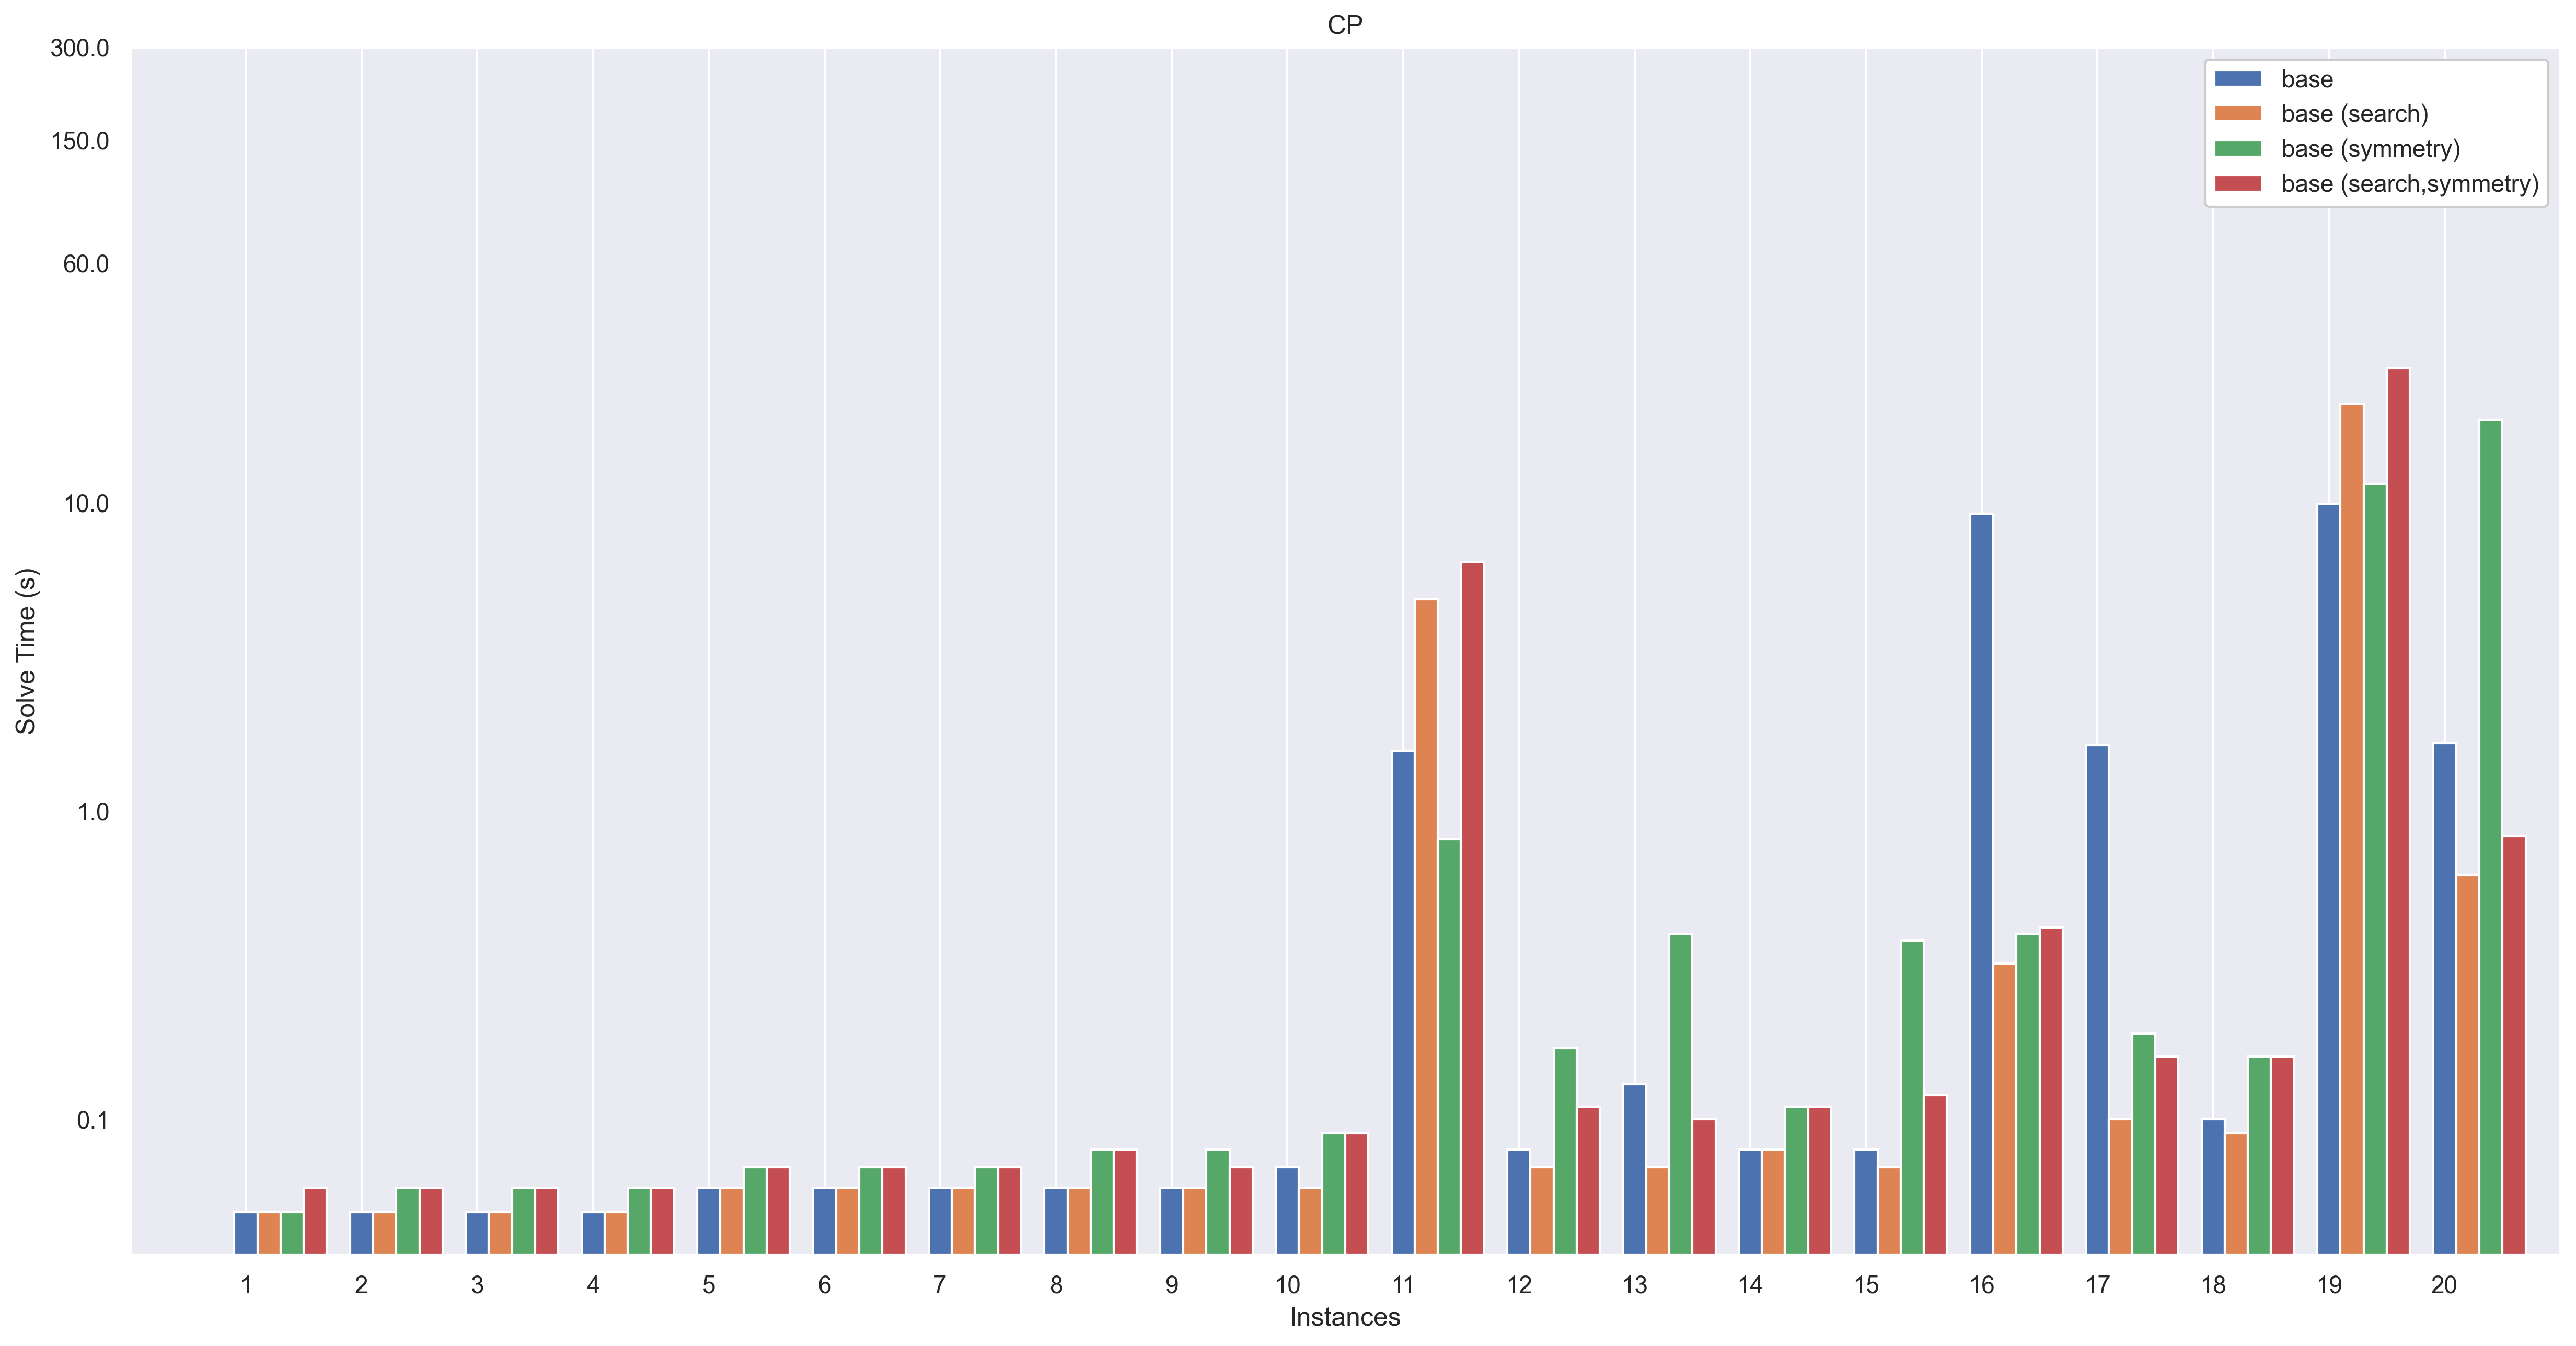
\includegraphics[width=1\textwidth]{03/results/base1.png}
  \caption{
    \colorbox{BurntOrange}{TODO missing ...}
  }
  \label{fig:CP_results_base1}
\end{figure}
\begin{figure}[H]
  \centering
  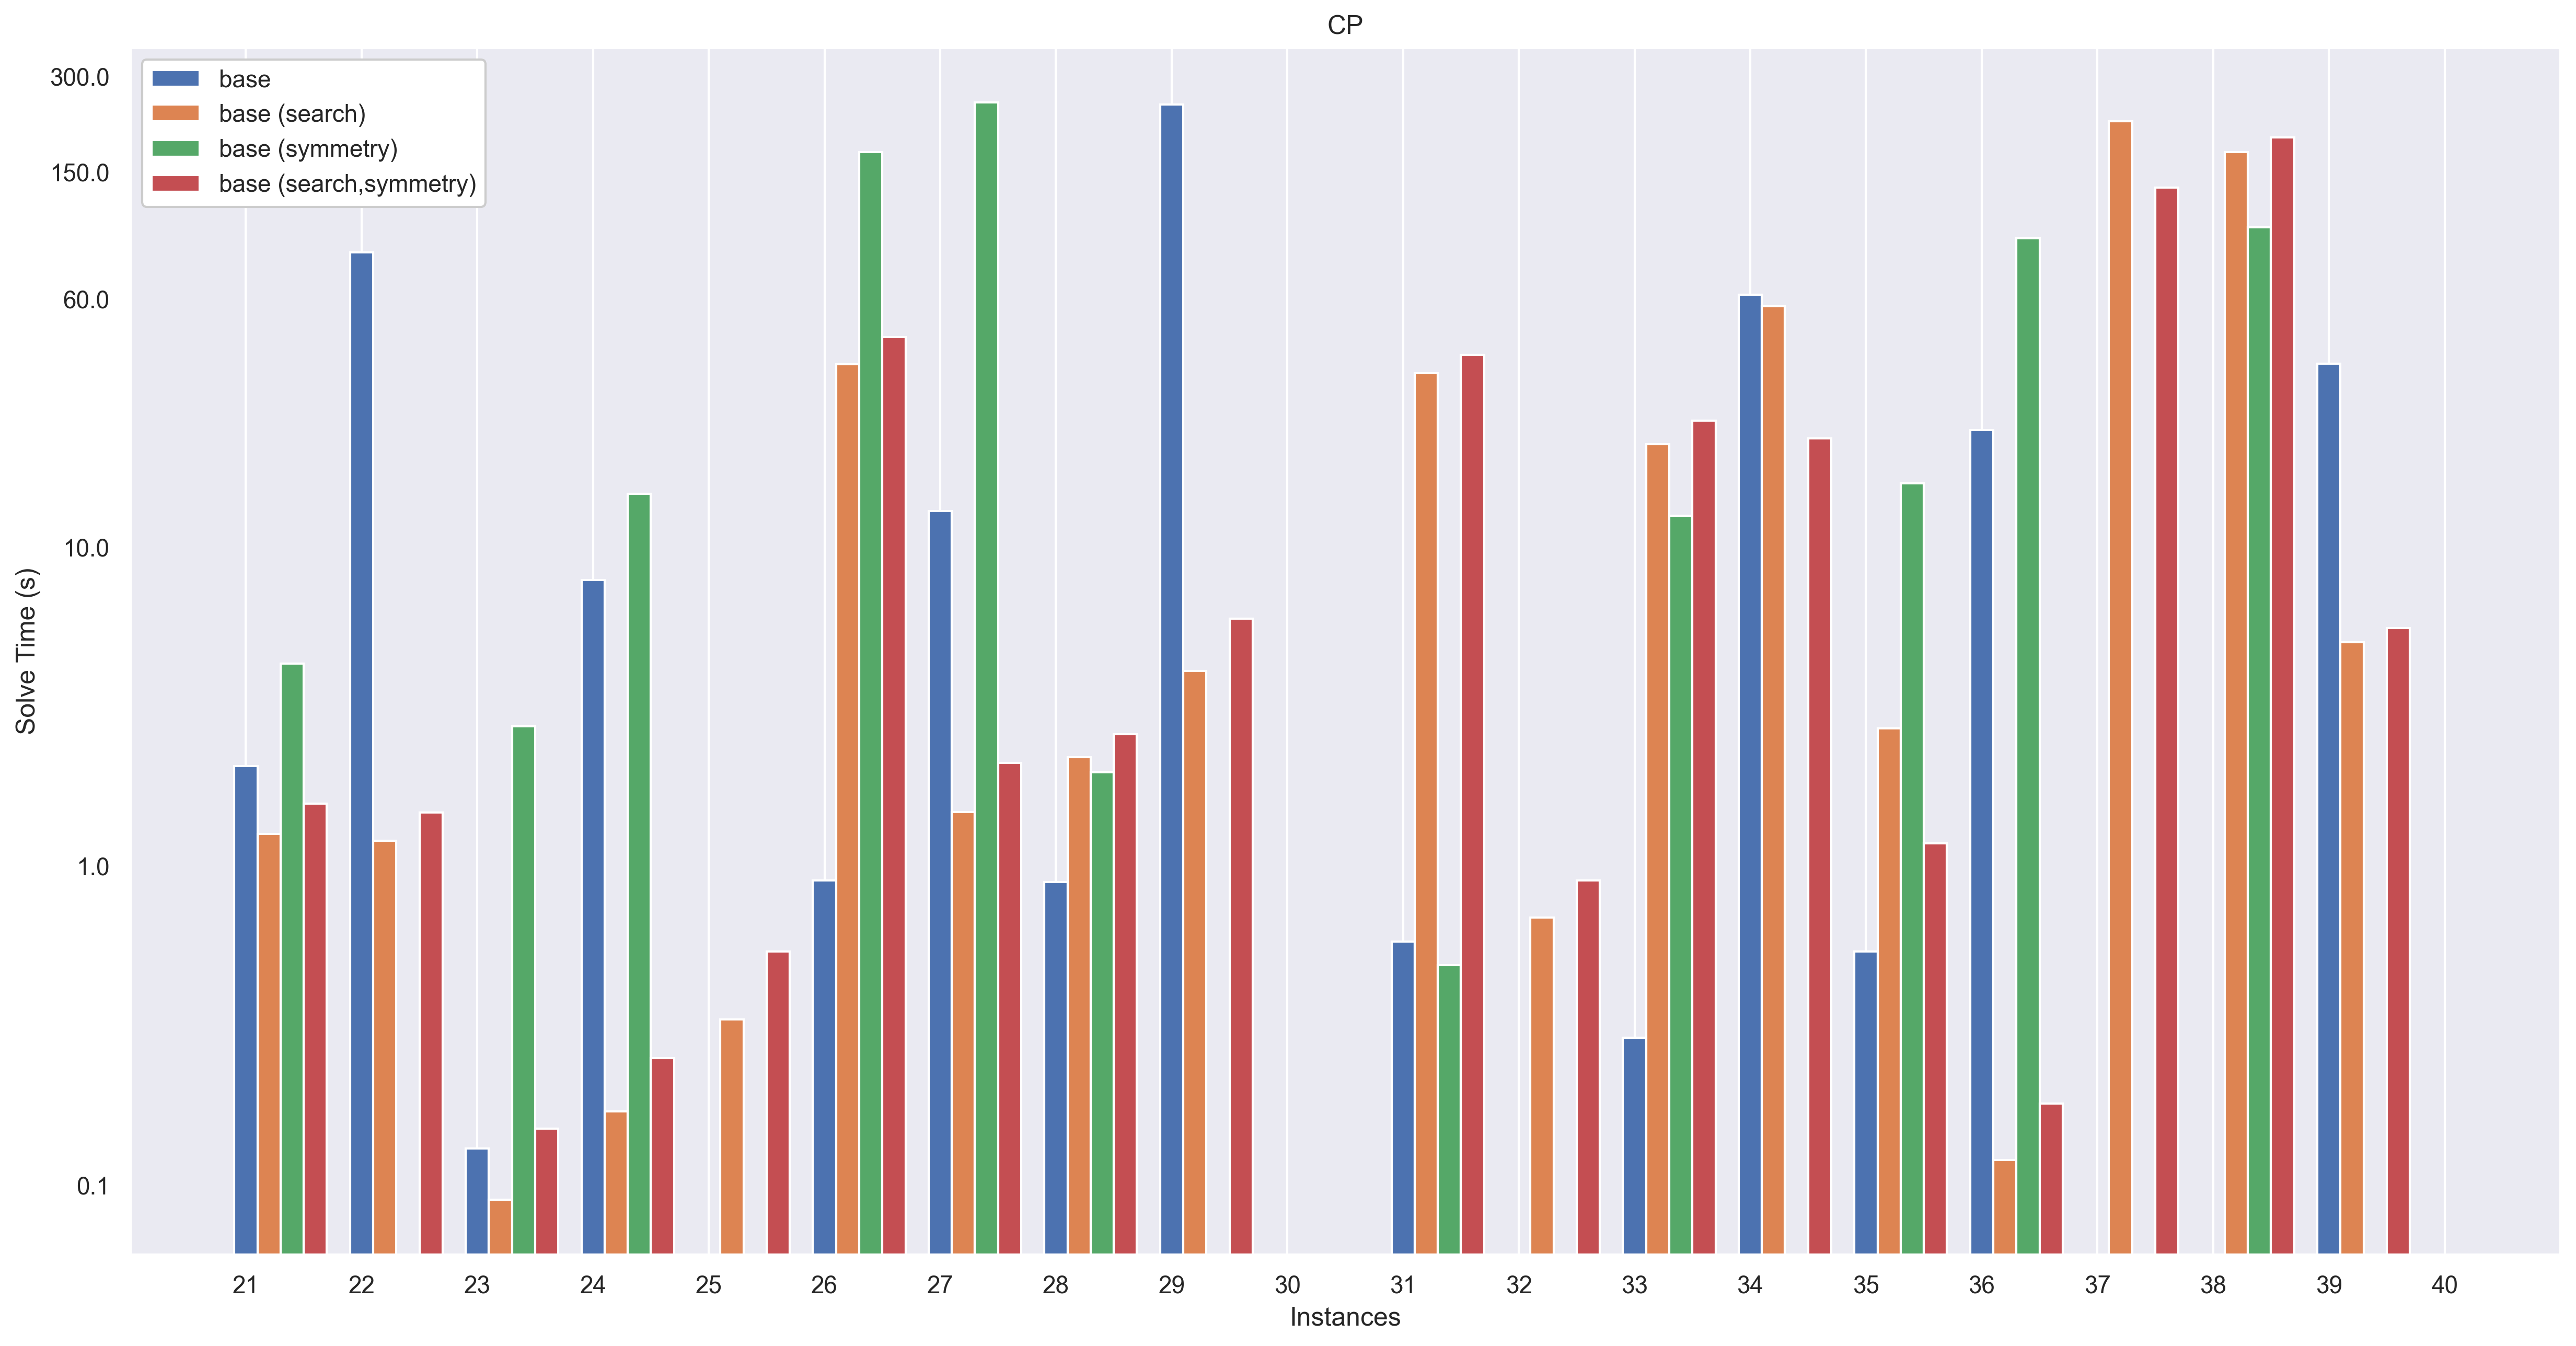
\includegraphics[width=1\textwidth]{03/results/base2.png}
  \caption{
    \colorbox{BurntOrange}{TODO missing ...}
  }
  \label{fig:CP_results_base2}
\end{figure}

\colorbox{BurntOrange}{TODO missing ...} \\
The results obtained for the \(rotation\) Model are presented in the Figures [\ref{fig:CP_results_rotation1},\ref{fig:CP_results_rotation2}].

\begin{figure}[H]
  \centering
  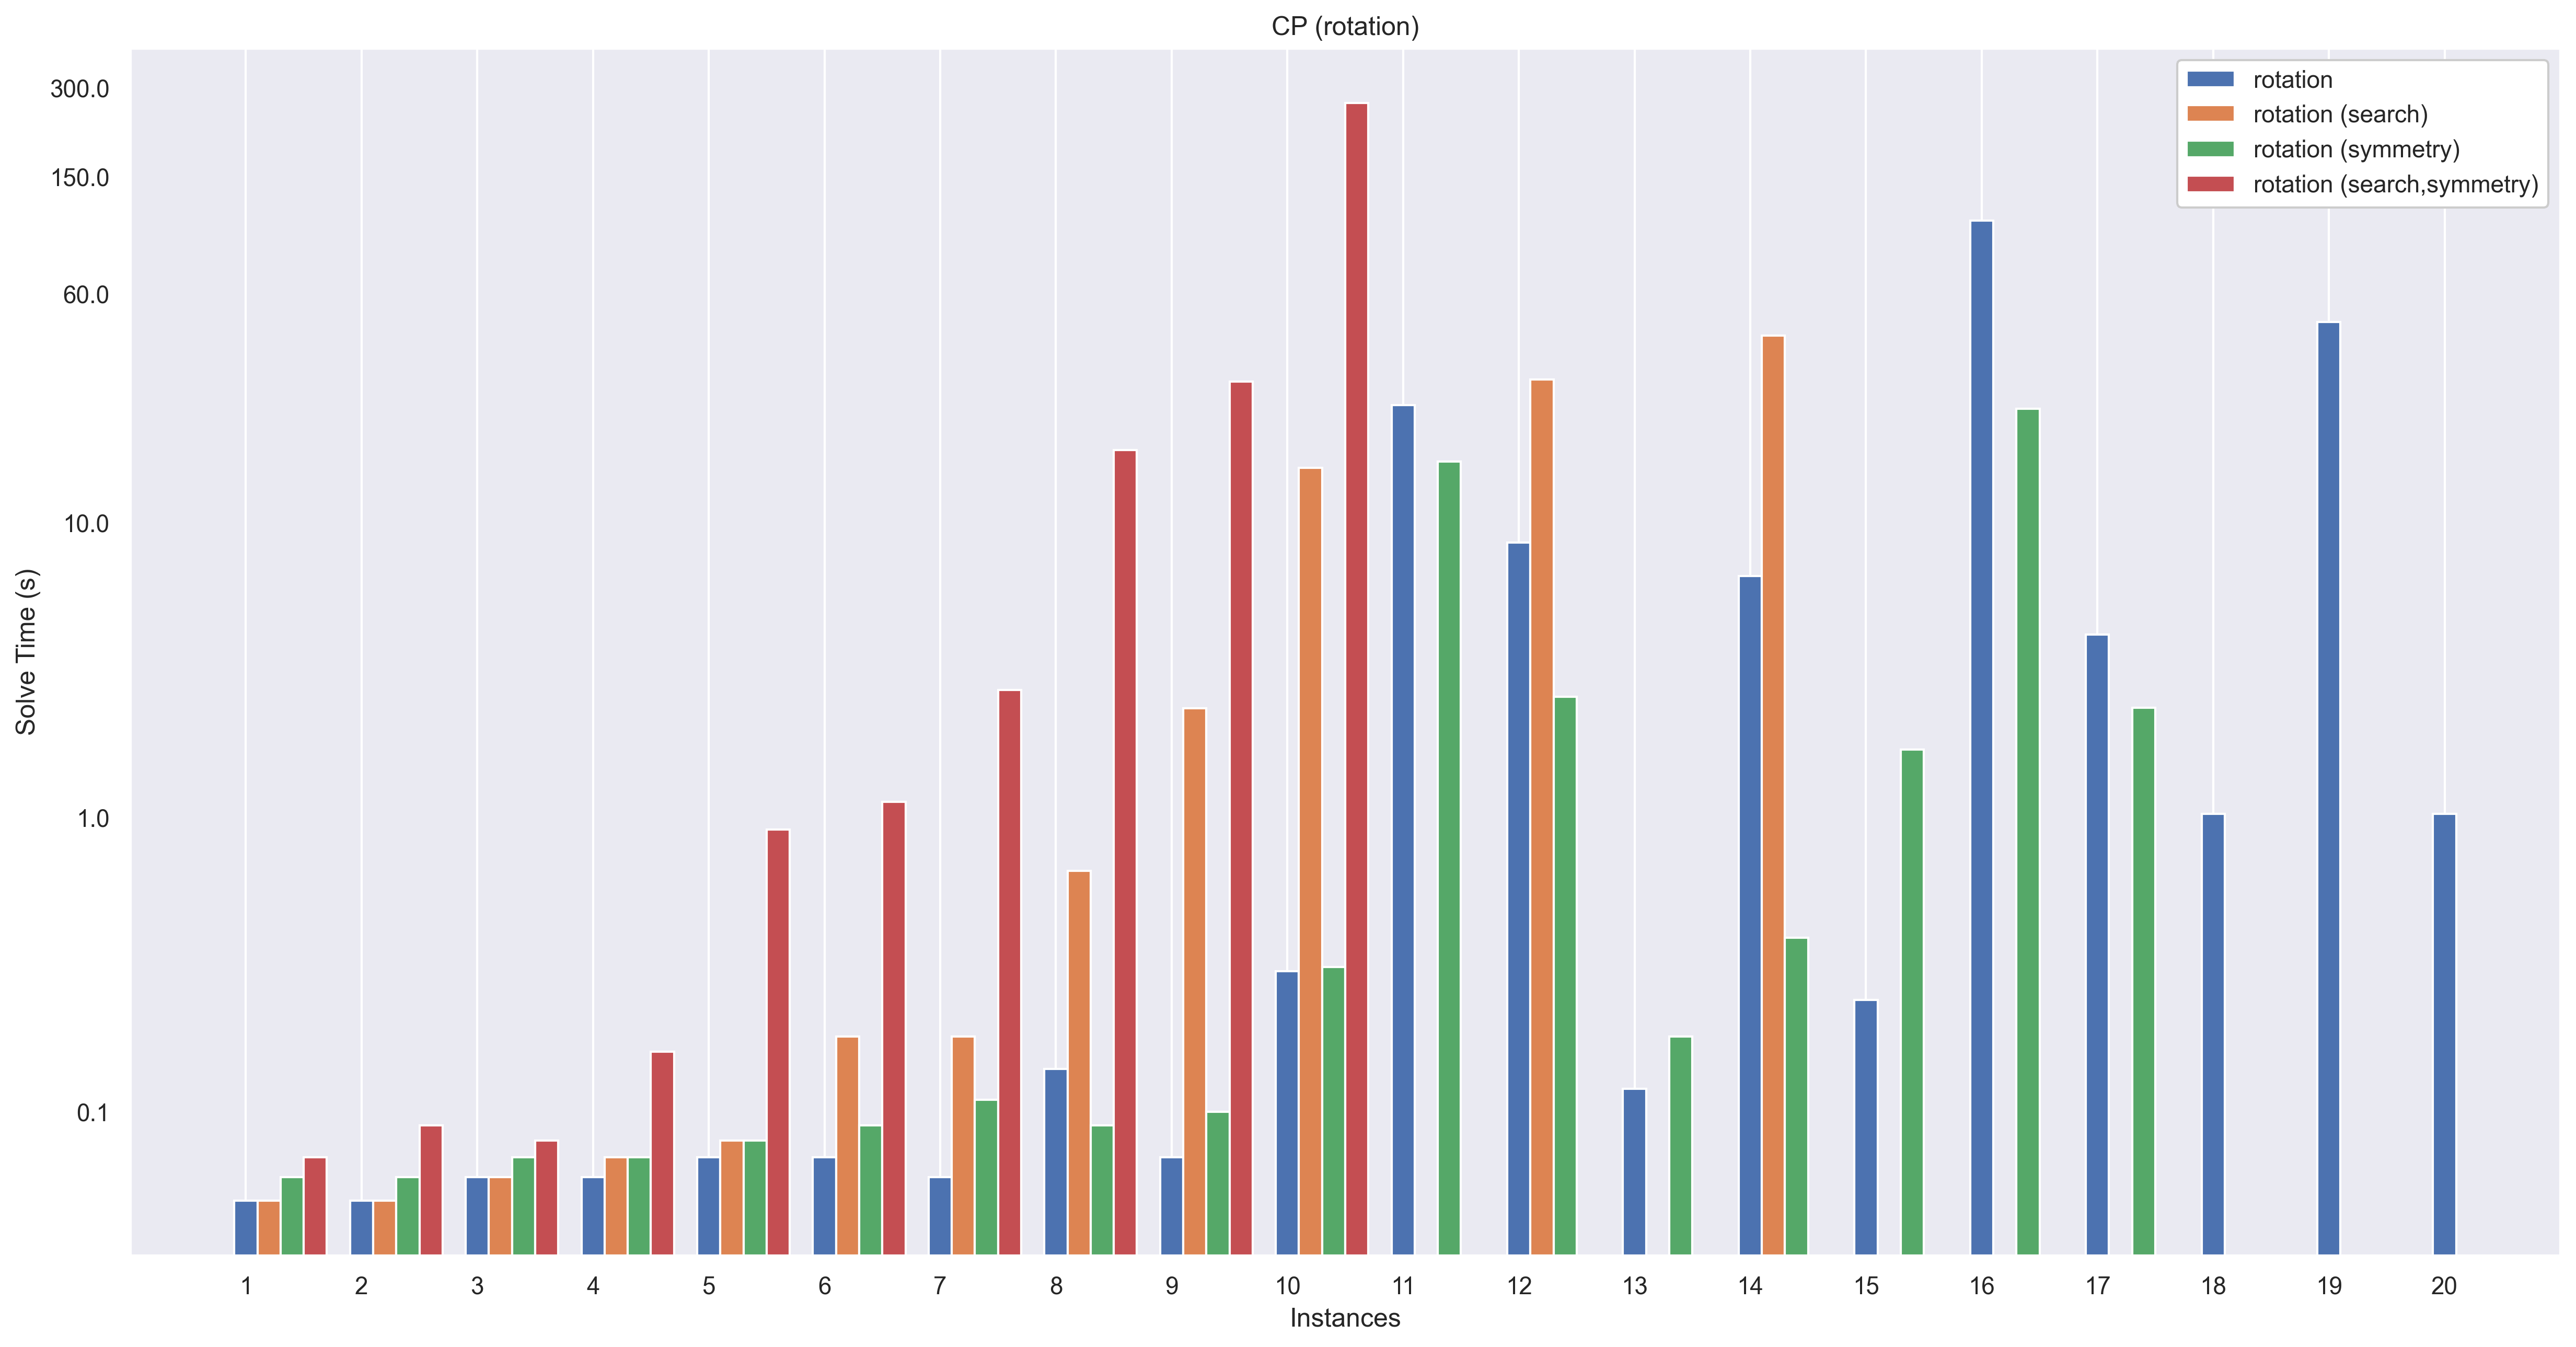
\includegraphics[width=1\textwidth]{03/results/rotation1.png}
  \caption{
    \colorbox{BurntOrange}{TODO missing ...}
  }
  \label{fig:CP_results_rotation1}
\end{figure}
\begin{figure}[H]
  \centering
  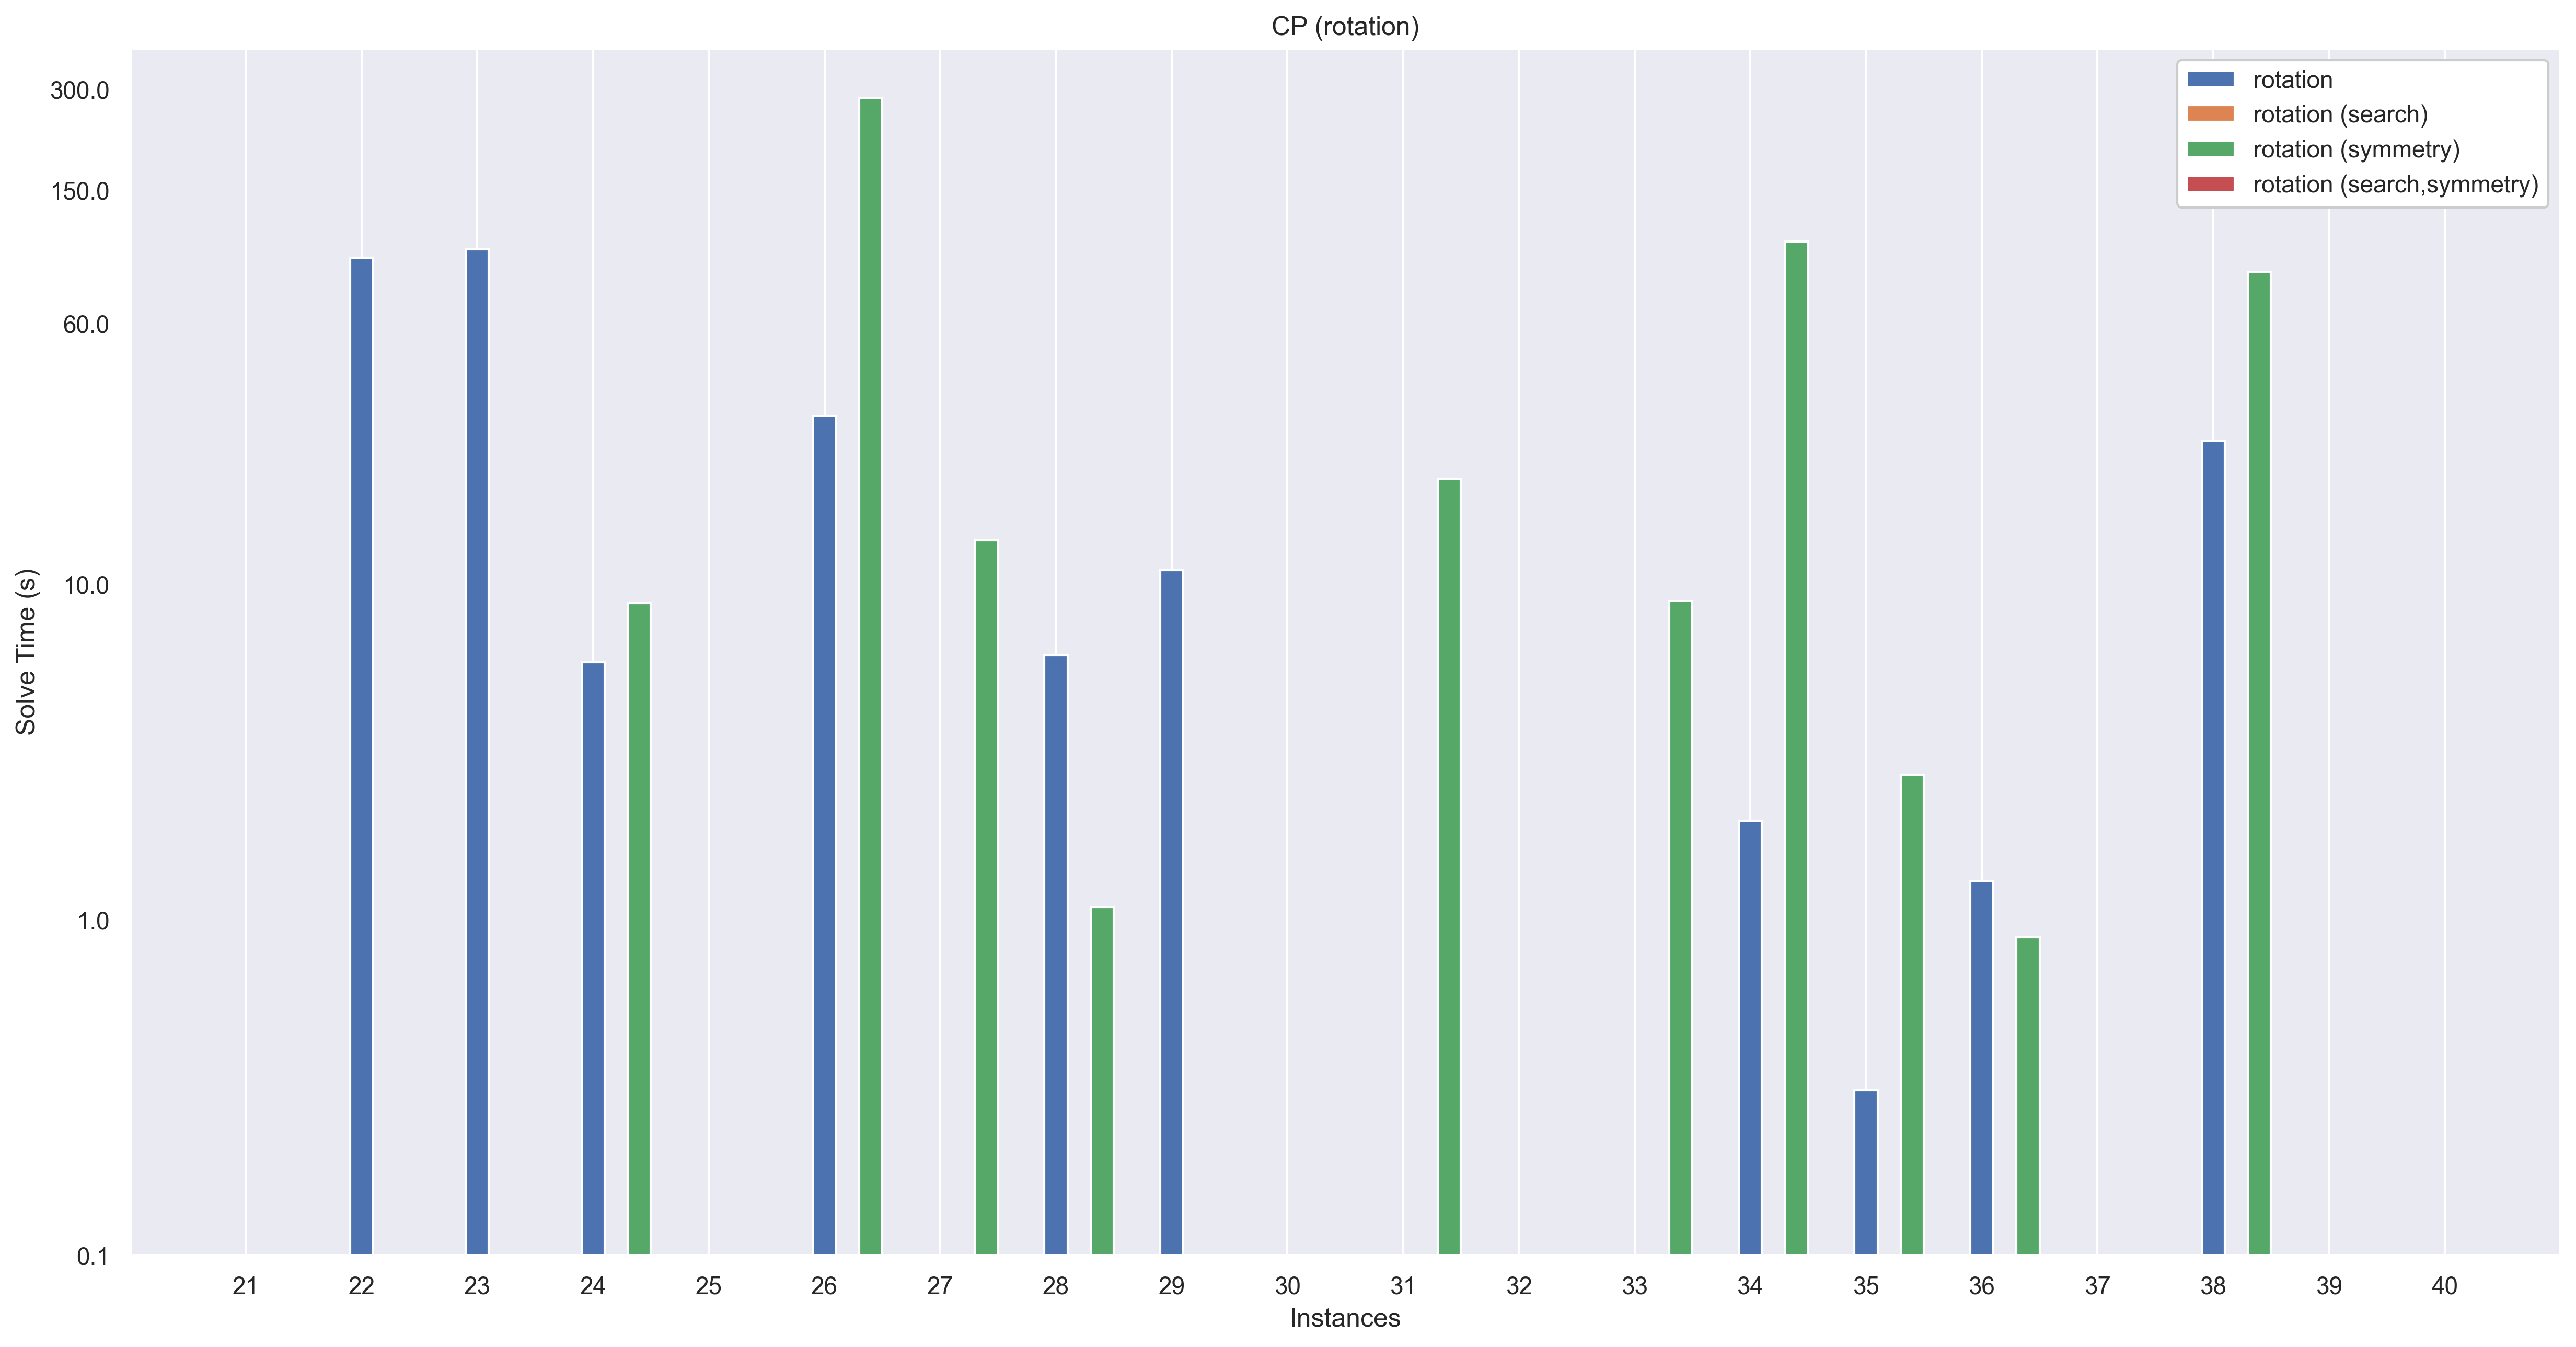
\includegraphics[width=1\textwidth]{03/results/rotation2.png}
  \caption{
    \colorbox{BurntOrange}{TODO missing ...}
  }
  \label{fig:CP_results_rotation2}
\end{figure}

